% Adjust these for the path of the theme and its graphics, relative to this file
%\usepackage{beamerthemeFalmouthGamesAcademy}
\usepackage{../../beamerthemeFalmouthGamesAcademy}
\usepackage{multimedia}
\graphicspath{ {../../} }

% Default language for code listings
\lstset{language=Python
}

% For strikethrough effect
\usepackage[normalem]{ulem}
\usepackage{wasysym}

\usepackage{pdfpages}

% http://www.texample.net/tikz/examples/state-machine/
\usetikzlibrary{arrows,automata}

\newcommand{\modulecode}{COMP260}\newcommand{\moduletitle}{Distributed Systems}\newcommand{\sessionnumber}{5}

\begin{document}
\title{\sessionnumber: Basic Principles for Computation}
\subtitle{\modulecode: \moduletitle}

\frame{\titlepage} 

\begin{frame}{Learning outcomes}
	By the end of today's session, you should be able to:
	\begin{itemize}
		\item Recall the historic significance of Alan Turing and his...
		\item Explain the basic concept of Turing Machines
		\item 
	\end{itemize}
\end{frame}

\begin{frame}{Agenda}
	\begin{itemize}
		\item The PyCharm IDE
		\item Basic Python programs
			\begin{itemize}
				\item Variable assignment
				\item Conditionals
				\item Loops
			\end{itemize}
		\item Coffee break
		\item SpaceChem worksheet review
	\end{itemize}
\end{frame}

\begin{frame}
	\begin{figure}
		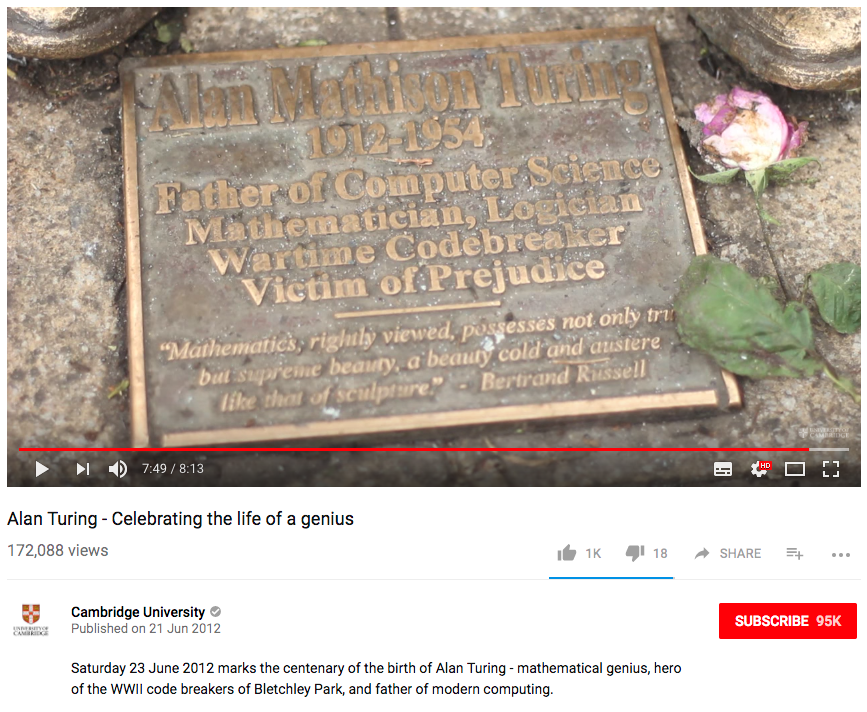
\includegraphics[scale=0.2]{assets/turingvideo.png}
		\caption{\href{https://www.youtube.com/watch?v=gtRLmL70TH0}{https://www.youtube.com/watch?v=gtRLmL70TH0}}
	\end{figure}
\end{frame}

\begin{frame}
	\frametitle{Activity - Groups of Six}
	\begin{figure}
		
\includegraphics[scale=0.3]{assets/activity.png}
	\end{figure}
\end{frame}

\begin{frame}

	\begin{figure}
		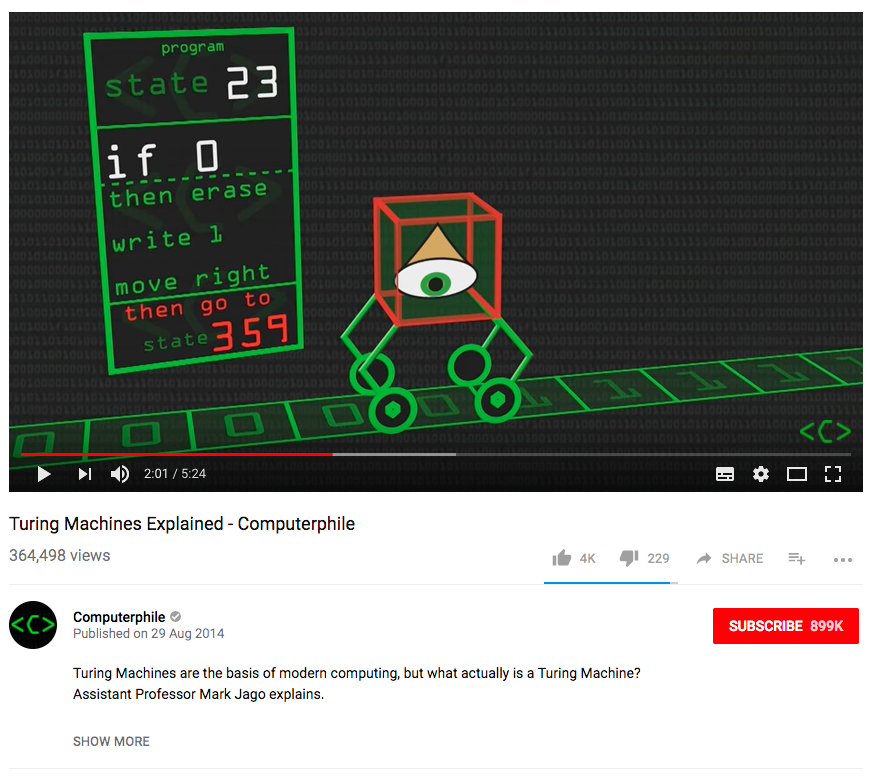
\includegraphics[scale=0.2]{assets/compute.png}
		\caption{\href{https://www.youtube.com/watch?v=dNRDvLACg5Q}{https://www.youtube.com/watch?v=dNRDvLACg5Q}}
	\end{figure}
\end{frame}

\begin{frame}
	\begin{figure}
		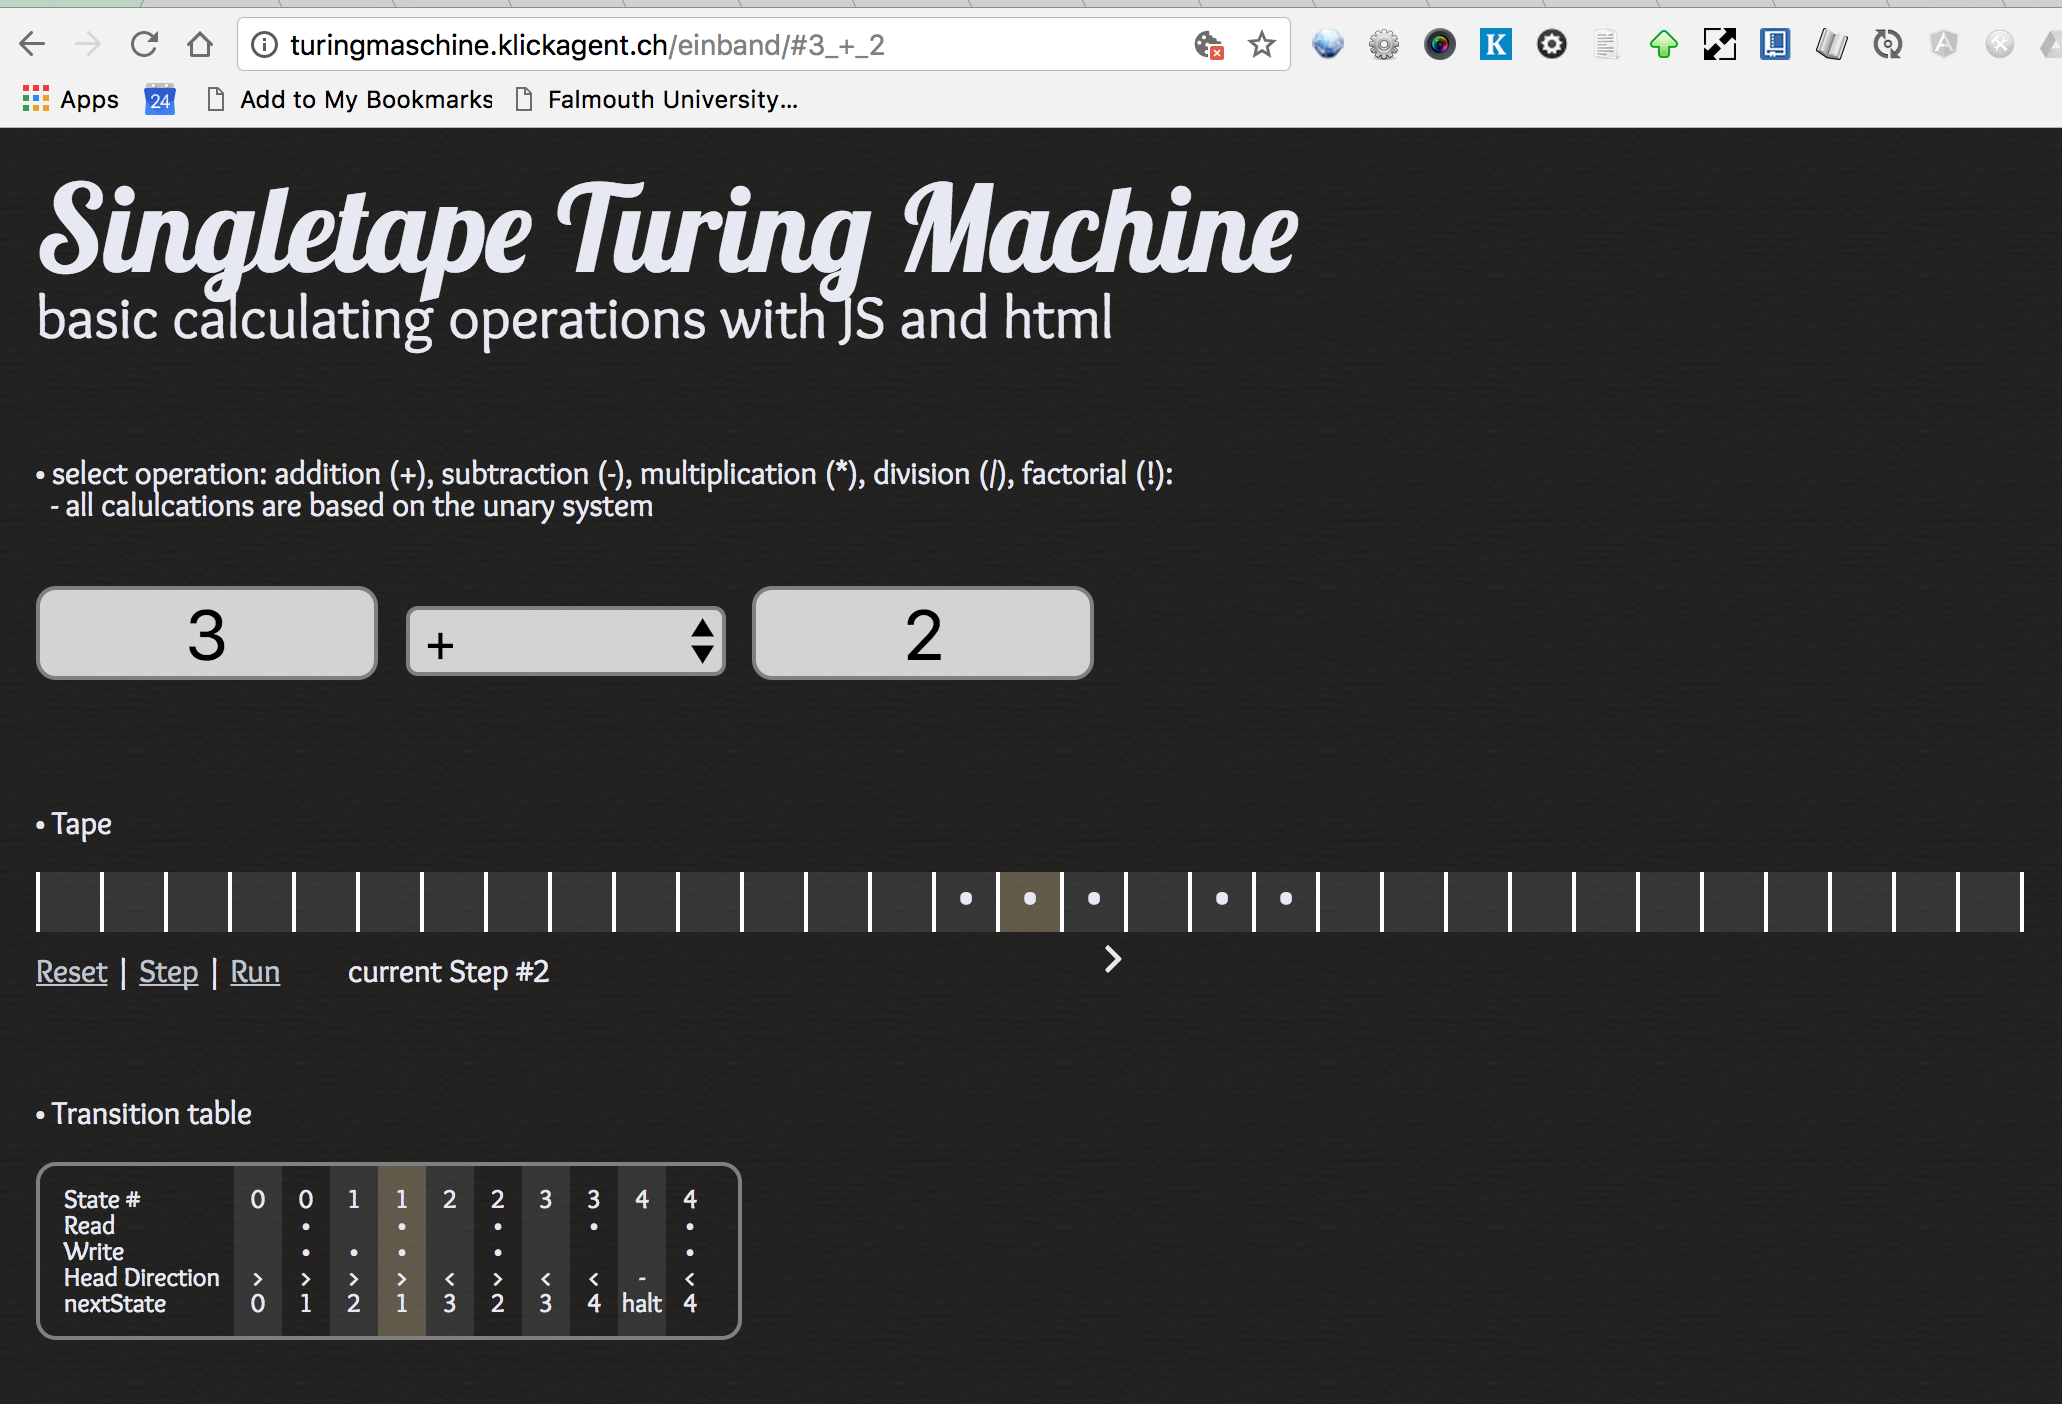
\includegraphics[scale=0.2]{assets/interactive.png}
		\caption{\href{http://turingmaschine.klickagent.ch/einband/}{http://turingmaschine.klickagent.ch/einband/}}
	\end{figure}
\end{frame}

\begin{frame}
	\frametitle{Turing Completeness}
	
	To show that something is Turing complete, it is enough to show that it can be used to simulate some Turing complete system. 	\\ ~ \\
	For an imperative language to be classed as Turing Complete it must have:

	\begin{itemize}
		\item Conditional branching (e.g., ``if'' and ``goto'' statements, or a ``branch if zero'' instruction)
		\item Ability to change an arbitrary amount of memory (e.g., the ability to maintain an arbitrary number of variables).
	\end{itemize}
\end{frame}

\begin{frame}
	!!! Since this is almost always the case, most if not all imperative languages are Turing complete if the limitations of finite memory are ignored.
\end{frame}


\end{document}
